\documentclass[border=5pt]{standalone}
\usepackage[T1]{fontenc}
\usepackage{lmodern}
\usepackage{pgfplots}
\usepgfplotslibrary{groupplots}
\pgfplotsset{compat=1.18}
\begin{document}\sffamily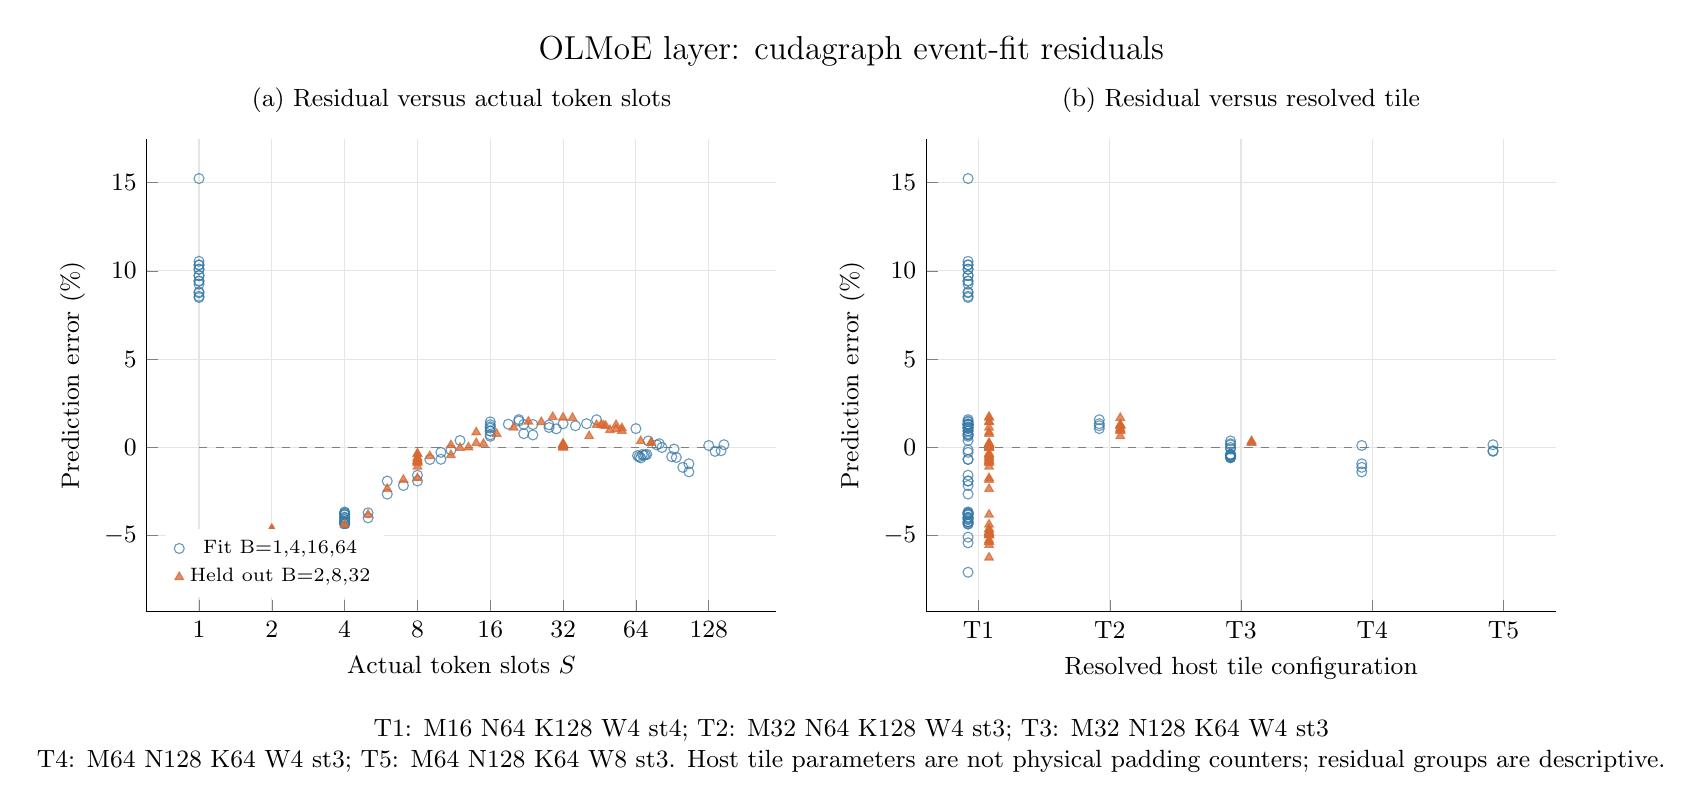
\begin{tikzpicture}
\definecolor{cal}{HTML}{3478A5}\definecolor{test}{HTML}{D76832}\definecolor{profile}{HTML}{3B8A5A}
\begin{groupplot}[group style={group size=2 by 1,horizontal sep=1.9cm},width=8.0cm,height=6.0cm,scale only axis,axis lines*=left,grid=major,grid style={gray!20},tick label style={font=\small},label style={font=\small},title style={font=\small},legend style={font=\scriptsize,draw=none},unbounded coords=jump]
\nextgroupplot[title={(a) Residual versus actual token slots},xlabel={Actual token slots $S$},ylabel={Prediction error (\%)},xmode=log,log basis x=2,xtick={1,2,4,8,16,32,64,128},xticklabels={1,2,4,8,16,32,64,128},legend pos=south west]\addplot[only marks,color=cal,mark=o,mark size=1.8pt,opacity=0.75] coordinates {(1,15.2341927244) (1,10.3280050002) (1,9.24996348318) (2,-5.40533580277) (1,8.81277411328) (1,8.75652098822) (3,-7.07289400915) (1,8.49232355062) (1,8.56451838833) (4,-5.08126215943) (1,9.43541211112) (1,10.3462782672) (5,-3.70696775414) (1,9.41594061791) (1,10.5446424106) (6,-2.6465267808) (1,9.73434707452) (1,10.0879530181) (7,-2.15613760148) (1,9.7403725901) (1,10.1000832168) (8,-1.90144295735) (4,-4.33889212308) (4,-4.27480591733) (5,-3.99081799458) (6,-1.90624939922) (4,-3.95398680465) (4,-3.65688979013) (8,-1.57495108733) (4,-4.34095267342) (4,-3.80408442166) (10,-0.281329191685) (4,-4.09930915337) (4,-3.81999048855) (12,0.394835388777) (4,-4.0485270407) (4,-3.97229215142) (9,-0.683312697438) (4,-4.21690003714) (4,-3.70659246037) (10,-0.671037785824) (4,-4.20750448825) (4,-3.75119189711) (11,-0.141235971308) (16,0.712711168398) (16,1.4497955489) (19,1.31507491854) (21,1.57626121488) (16,1.16879244377) (22,0.778274756674) (24,1.29698078639) (16,0.929369779935) (22,1.30456383474) (28,1.27753838488) (16,0.929877401074) (24,0.707164468029) (32,1.34027045214) (16,0.627821241194) (21,1.49595392905) (36,1.22722774777) (16,1.28418455486) (28,1.12908621313) (40,1.34359805146) (16,1.09311322833) (30,1.05213077869) (44,1.56583551349) (64,1.06785863459) (65,-0.465712125439) (72,0.366003702855) (78,0.145960142141) (66,-0.528405420391) (80,0.208622191693) (90,-0.524684751543) (67,-0.594645475926) (82,-0.0026450164709) (106,-0.927294491412) (68,-0.398310805908) (92,-0.0938181064211) (128,0.110476699974) (69,-0.448205845681) (94,-0.570942633411) (144,-0.18633427101) (70,-0.427204983721) (100,-1.12935603) (136,-0.223845456427) (71,-0.391013710857) (106,-1.38716975501) (148,0.15255765905)};
\addlegendentry{Fit B=1,4,16,64}
\addplot[only marks,color=test,mark=triangle*,mark size=1.8pt,opacity=0.75] coordinates {(2,-5.52434756066) (2,-4.81485432114) (2,-5.32958046413) (3,-6.2379114898) (2,-4.87324792915) (2,-4.84747308801) (4,-4.36751841368) (2,-5.23941604153) (2,-4.96486751656) (5,-3.80792662032) (2,-5.34984294459) (2,-4.97469911811) (6,-2.34991156117) (2,-4.9285429751) (2,-4.6384782553) (7,-1.83022738668) (2,-4.75334873032) (2,-4.6209575047) (8,-1.73906612884) (2,-4.93535591959) (2,-4.85733040492) (9,-0.491564576547) (8,-0.761490905055) (8,-0.619071825818) (8,-0.364071682665) (11,0.131013207999) (8,-0.567965863731) (8,-0.353104546294) (14,0.856687160831) (8,-0.815844032691) (11,-0.432016394348) (17,0.769603590769) (8,-0.871512016249) (12,-0.0218480217453) (20,1.12927973347) (8,-0.764971310644) (13,0.00674562155173) (23,1.46639865067) (8,-0.678665664284) (14,0.245987635454) (26,1.439202928) (8,-1.08455127166) (15,0.208418080299) (29,1.72586878126) (32,1.69518116881) (32,0.0760999618162) (41,0.643331183372) (35,1.67661604106) (32,0.183429550948) (46,1.28884074324) (48,1.21734526113) (32,0.206889662959) (50,0.98806848031) (53,1.03346745821) (32,0.14857530191) (56,0.941647002946) (44,1.27320038073) (32,0.0109883775614) (47,1.24953497669) (67,0.356778735982) (32,0.0577575428671) (56,1.09125293245) (74,0.286107517041) (32,-0.0123795192011) (74,0.254860375315) (53,1.2686406456)};
\addlegendentry{Held out B=2,8,32}\addplot[gray,dashed,forget plot,domain=1:148] {0};
\nextgroupplot[title={(b) Residual versus resolved tile},xlabel={Resolved host tile configuration},ylabel={Prediction error (\%)},xtick={1,2,3,4,5},xticklabels={T1,T2,T3,T4,T5},xmin=0.6,xmax=5.4]\addplot[only marks,color=cal,mark=o,mark size=1.8pt,opacity=0.75] coordinates {(0.92,15.2341927244) (0.92,10.3280050002) (0.92,9.24996348318) (0.92,-5.40533580277) (0.92,8.81277411328) (0.92,8.75652098822) (0.92,-7.07289400915) (0.92,8.49232355062) (0.92,8.56451838833) (0.92,-5.08126215943) (0.92,9.43541211112) (0.92,10.3462782672) (0.92,-3.70696775414) (0.92,9.41594061791) (0.92,10.5446424106) (0.92,-2.6465267808) (0.92,9.73434707452) (0.92,10.0879530181) (0.92,-2.15613760148) (0.92,9.7403725901) (0.92,10.1000832168) (0.92,-1.90144295735) (0.92,-4.33889212308) (0.92,-4.27480591733) (0.92,-3.99081799458) (0.92,-1.90624939922) (0.92,-3.95398680465) (0.92,-3.65688979013) (0.92,-1.57495108733) (0.92,-4.34095267342) (0.92,-3.80408442166) (0.92,-0.281329191685) (0.92,-4.09930915337) (0.92,-3.81999048855) (0.92,0.394835388777) (0.92,-4.0485270407) (0.92,-3.97229215142) (0.92,-0.683312697438) (0.92,-4.21690003714) (0.92,-3.70659246037) (0.92,-0.671037785824) (0.92,-4.20750448825) (0.92,-3.75119189711) (0.92,-0.141235971308) (0.92,0.712711168398) (0.92,1.4497955489) (0.92,1.31507491854) (0.92,1.57626121488) (0.92,1.16879244377) (0.92,0.778274756674) (0.92,1.29698078639) (0.92,0.929369779935) (0.92,1.30456383474) (0.92,1.27753838488) (0.92,0.929877401074) (0.92,0.707164468029) (0.92,1.34027045214) (0.92,0.627821241194) (0.92,1.49595392905) (1.92,1.22722774777) (0.92,1.28418455486) (0.92,1.12908621313) (1.92,1.34359805146) (0.92,1.09311322833) (0.92,1.05213077869) (1.92,1.56583551349) (1.92,1.06785863459) (2.92,-0.465712125439) (2.92,0.366003702855) (2.92,0.145960142141) (2.92,-0.528405420391) (2.92,0.208622191693) (2.92,-0.524684751543) (2.92,-0.594645475926) (2.92,-0.0026450164709) (3.92,-0.927294491412) (2.92,-0.398310805908) (2.92,-0.0938181064211) (3.92,0.110476699974) (2.92,-0.448205845681) (2.92,-0.570942633411) (4.92,-0.18633427101) (2.92,-0.427204983721) (3.92,-1.12935603) (4.92,-0.223845456427) (2.92,-0.391013710857) (3.92,-1.38716975501) (4.92,0.15255765905)};
\addplot[only marks,color=test,mark=triangle*,mark size=1.8pt,opacity=0.75] coordinates {(1.08,-5.52434756066) (1.08,-4.81485432114) (1.08,-5.32958046413) (1.08,-6.2379114898) (1.08,-4.87324792915) (1.08,-4.84747308801) (1.08,-4.36751841368) (1.08,-5.23941604153) (1.08,-4.96486751656) (1.08,-3.80792662032) (1.08,-5.34984294459) (1.08,-4.97469911811) (1.08,-2.34991156117) (1.08,-4.9285429751) (1.08,-4.6384782553) (1.08,-1.83022738668) (1.08,-4.75334873032) (1.08,-4.6209575047) (1.08,-1.73906612884) (1.08,-4.93535591959) (1.08,-4.85733040492) (1.08,-0.491564576547) (1.08,-0.761490905055) (1.08,-0.619071825818) (1.08,-0.364071682665) (1.08,0.131013207999) (1.08,-0.567965863731) (1.08,-0.353104546294) (1.08,0.856687160831) (1.08,-0.815844032691) (1.08,-0.432016394348) (1.08,0.769603590769) (1.08,-0.871512016249) (1.08,-0.0218480217453) (1.08,1.12927973347) (1.08,-0.764971310644) (1.08,0.00674562155173) (1.08,1.46639865067) (1.08,-0.678665664284) (1.08,0.245987635454) (1.08,1.439202928) (1.08,-1.08455127166) (1.08,0.208418080299) (1.08,1.72586878126) (1.08,1.69518116881) (1.08,0.0760999618162) (2.08,0.643331183372) (2.08,1.67661604106) (1.08,0.183429550948) (2.08,1.28884074324) (2.08,1.21734526113) (1.08,0.206889662959) (2.08,0.98806848031) (2.08,1.03346745821) (1.08,0.14857530191) (2.08,0.941647002946) (2.08,1.27320038073) (1.08,0.0109883775614) (2.08,1.24953497669) (3.08,0.356778735982) (1.08,0.0577575428671) (2.08,1.09125293245) (3.08,0.286107517041) (1.08,-0.0123795192011) (3.08,0.254860375315) (2.08,1.2686406456)};\addplot[gray,dashed,forget plot,domain=1:5] {0};
\end{groupplot}
\path (group c1r1.north west) -- node[above=0.8cm,font=\large] {OLMoE layer: cudagraph event-fit residuals} (group c2r1.north east);
\path (group c1r1.south west) -- node[below=1.25cm,align=center,font=\small] {T1: M16 N64 K128 W4 st4; T2: M32 N64 K128 W4 st3; T3: M32 N128 K64 W4 st3\\T4: M64 N128 K64 W4 st3; T5: M64 N128 K64 W8 st3. Host tile parameters are not physical padding counters; residual groups are descriptive.} (group c2r1.south east);
\end{tikzpicture}\end{document}
